%%%%%%%%%%%%%%%%%%%%%%%%%%%%%%%%%%%%%%%%%
% Programming/Coding Assignment
% LaTeX Template
%
% This template has been downloaded from:
% http://www.latextemplates.com
%
% Original author:
% Ted Pavlic (http://www.tedpavlic.com)
%
% Note:
% The \lipsum[#] commands throughout this template generate dummy text
% to fill the template out. These commands should all be removed when 
% writing assignment content.
%
% This template uses a Perl script as an example snippet of code, most other
% languages are also usable. Configure them in the "CODE INCLUSION 
% CONFIGURATION" section.
%
%%%%%%%%%%%%%%%%%%%%%%%%%%%%%%%%%%%%%%%%%

%----------------------------------------------------------------------------------------
%	PACKAGES AND OTHER DOCUMENT CONFIGURATIONS
%----------------------------------------------------------------------------------------

\documentclass[a4paper]{article}
\usepackage[utf8]{inputenc}
\usepackage{listingsutf8}
\usepackage[spanish]{babel}




\usepackage{fancyhdr} % Required for custom headers
\usepackage{lastpage} % Required to determine the last page for the footer
\usepackage{extramarks} % Required for headers and footers
\usepackage[usenames,dvipsnames]{color} % Required for custom colors
\usepackage{graphicx} % Required to insert images
\usepackage{listings} % Required for insertion of code
\usepackage{courier} % Required for the courier font
\usepackage{lipsum} % Used for inserting dummy 'Lorem ipsum' text into the template
\usepackage{svg}
\usepackage{attachfile}
\usepackage{currfile}
\usepackage{multicol}
\usepackage{alltt}
\usepackage{framed}
\usepackage{caption}
\usepackage{seqsplit}

\hypersetup{
colorlinks,
citecolor=black,
filecolor=black,
linkcolor=black,
urlcolor=blue
}


% Margins
\topmargin=-0.45in
\evensidemargin=0in
\oddsidemargin=0in
\textwidth=6.5in
\textheight=9.8in
\headsep=0.25in

\linespread{1.1} % Line spacing
\setlength{\parindent}{1.5em}
\setlength{\parskip}{1em}


% Set up the header and footer
\pagestyle{fancy}
%\lhead{\hmwkAuthorName} % Top left header
\lhead{\hmwkClass}
\rhead{\hmwkTitle} % Top right header
\chead{} % Top center head
\lfoot{\lastxmark} % Bottom left footer
\cfoot{} % Bottom center footer
\rfoot{ \thepage\ / \protect\pageref{LastPage}} % Bottom right footer
\renewcommand\headrulewidth{0.4pt} % Size of the header rule
\renewcommand\footrulewidth{0.4pt} % Size of the footer rule



%----------------------------------------------------------------------------------------
%	CODE INCLUSION CONFIGURATION
%----------------------------------------------------------------------------------------
\renewcommand{\ttdefault}{pcr}
\definecolor{MyDarkGreen}{rgb}{0.0,0.4,0.0} % This is the color used for comments
\lstloadlanguages{Perl} % Load Perl syntax for listings, for a list of other languages supported see: ftp://ftp.tex.ac.uk/tex-archive/macros/latex/contrib/listings/listings.pdf
\lstset{
language=sh, % Use Perl in this example
frame=single, % Single frame around code
basicstyle=\small\ttfamily, % Use small true type font
keywordstyle=[1]\small\color{Blue}\bf, % Perl functions bold and blue
keywordstyle=[2]\small\color{Purple}, % Perl function arguments purple
keywordstyle=[3]\small\color{Blue}\underbar, % Custom functions underlined and blue
identifierstyle=, % Nothing special about identifiers                                         
commentstyle=\small\color{MyDarkGreen}, % Comments small dark green courier font
stringstyle=\small\color{Purple}, % Strings are purple
showstringspaces=false, % Don't put marks in string spaces
tabsize=5, % 5 spaces per tab
morecomment=[l][\small\color{Blue}]{...}, % Line continuation (...) like blue comment
numbers=none, % Line numbers on left
firstnumber=1, % Line numbers start with line 1
numberstyle=\tiny\color{Blue}, % Line numbers are blue and small
stepnumber=0 % Line numbers go in steps of 5
}

% Creates a new command to include a perl script, the first parameter is the filename of the script (without .pl), the second parameter is the caption
\newcommand{\perlscript}[2]{
\begin{itemize}
\item[]\lstinputlisting[caption=#2,label=#1]{#1.pl}
\end{itemize}
}

%----------------------------------------------------------------------------------------
%	DOCUMENT STRUCTURE COMMANDS
%	Skip this unless you know what you're doing
%----------------------------------------------------------------------------------------

% Header and footer for when a page split occurs within a problem environment
\newcommand{\enterProblemHeader}[1]{
%\nobreak\extramarks{#1}{#1 continued on next page\ldots}\nobreak
%\nobreak\extramarks{#1 (continued)}{#1 continued on next page\ldots}\nobreak
}

% Header and footer for when a page split occurs between problem environments
\newcommand{\exitProblemHeader}[1]{
%\nobreak\extramarks{#1 (continued)}{#1 continued on next page\ldots}\nobreak
%\nobreak\extramarks{#1}{}\nobreak
}

\setcounter{secnumdepth}{0} % Removes default section numbers
\newcounter{homeworkProblemCounter} % Creates a counter to keep track of the number of problems

\newcommand{\homeworkProblemName}{}
\newenvironment{homeworkProblem}[1][]{ % Makes a new environment called homeworkProblem which takes 1 argument (custom name) but the default is "Problem #"
\stepcounter{homeworkProblemCounter} % Increase counter for number of problems
\renewcommand{\homeworkProblemName}{Ejercicio \arabic{homeworkProblemCounter} #1} % Assign \homeworkProblemName the name of the problem
\section{\homeworkProblemName} % Make a section in the document with the custom problem count
\enterProblemHeader{\homeworkProblemName} % Header and footer within the environment
}{
\exitProblemHeader{\homeworkProblemName} % Header and footer after the environment
%\clearpage
}


\newcommand{\problemAnswer}[1]{ % Defines the problem answer command with the content as the only argument
\noindent\framebox[\columnwidth][c]{\begin{minipage}{0.98\columnwidth}#1\end{minipage}} % Makes the box around the problem answer and puts the content inside
}

\newcommand{\homeworkSectionName}{}
\newenvironment{homeworkSection}[1]{ % New environment for sections within homework problems, takes 1 argument - the name of the section
\renewcommand{\homeworkSectionName}{#1} % Assign \homeworkSectionName to the name of the section from the environment argument
\subsection{\homeworkSectionName} % Make a subsection with the custom name of the subsection
\enterProblemHeader{\homeworkProblemName\ [\homeworkSectionName]} % Header and footer within the environment
}{
\enterProblemHeader{\homeworkProblemName} % Header and footer after the environment
}

%----------------------------------------------------------------------------------------
%	NAME AND CLASS SECTION
%----------------------------------------------------------------------------------------

\newcommand{\hmwkTitle}{Redefine el hmwkTitle} % Assignment title
\newcommand{\hmwkDueDate}{asdfadsf} % Due date
\newcommand{\hmwkClass}{Redefine hmwkClass} % Course/class
\newcommand{\hmwkClassTime}{} % Class/lecture time
\newcommand{\hmwkClassInstructor}{} % Teacher/lecturer
\newcommand{\hmwkAuthorName}{Álvaro González Sotillo} % Your name

%----------------------------------------------------------------------------------------
%	TITLE PAGE
%----------------------------------------------------------------------------------------

\title{
\vspace{2in}
\textmd{\textbf{\hmwkClass:\ \hmwkTitle}}\\
\vspace{0.1in}\large{\textit{\hmwkClassInstructor\ \hmwkClassTime}}
\vspace{3in}
}

\author{\textbf{\hmwkAuthorName}}
\date{} % Insert date here if you want it to appear below your name


%----------------------------------------------------------------------------------------

\usepackage{fancybox}
\newcommand{\codigo}[1]{\texttt{#1}}


% CUADRITO
\newsavebox{\fmboxx}
\newenvironment{cuadrito}[1][14cm]
{\noindent \begin{center} \begin{lrbox}{\fmboxx}\noindent\begin{minipage}{#1}}
{\end{minipage}\end{lrbox}\noindent\shadowbox{\usebox{\fmboxx}} \end{center}}





\newenvironment{entradasalida}[2][14cm]
{
  \newcommand{\elnombredelafiguradeentradasalida}{#2}
  \begin{figure}[h]
    \begin{cuadrito}[#1]
      \begin{scriptsize}
\begin{alltt}
}
{%
\end{alltt}%
      \end{scriptsize}%
    \end{cuadrito}%
    \caption{\elnombredelafiguradeentradasalida}
  \end{figure}
}


\newenvironment{entradasalidacols}[2][14cm]
{
\newcommand{\elnombredelafiguradeentradasalida}{#2}
%\begin{wrapfigure}{}{0.1}
\begin{cuadrito}[#1]
\begin{scriptsize}
\begin{alltt}
}
{
\end{alltt}
\end{scriptsize}
\end{cuadrito}
\captionof{figure}{\elnombredelafiguradeentradasalida}
%\end{wrapfigure}
}


\usepackage{pgffor}
\newcommand{\ficheroautoref}[0]{%
  \foreach \ficherotex in {../../../common/plantilla-ejercicio.tex,../../common/plantilla-ejercicio.tex,../common/plantilla-ejercicio.tex,../apuntes/common/plantilla-ejercicio.tex}{

    \IfFileExists{\ficherotex}%
    {%
      \textattachfile[mimetype=text/plain,%
      description={La plantilla},%
      subject={La plantilla}]%
      {\ficherotex}%
      {}%
      % RECUPERO ESPACIO VERTICAL PERDIDO
      \vspace{-6em}%
    }%
    {}%
  }
  

  \textattachfile[mimetype=text/plain,
  description={El fichero TEX original para crear este documento, no sea que se nos pierda},
  subject={El fichero TEX original para crear este documento, no sea que se nos pierda}]
  {\currfilename}{}

}

\newcommand{\entradausuario}[1]{\textit{\textbf{#1}}}

\newcommand{\enlace}[2]{\textcolor{blue}{{\href{#1}{#2}}}}

\newcommand{\adjuntarfichero}[3]{
\textattachfile[mimetype=text/plain,
color={0 0 0},
description={#3},
subject={#1}]
{#1}
{\textcolor{blue}{\codigo{#2}}}
}

\newcommand{\adjuntardoc}[2]{%
\textattachfile[mimetype=text/plain,%
color={0 0 0},%
description={#1},%
subject={#1}]%
{#1}%
{\textcolor{blue}{#2}}%
}%


\newcommand{\plantilladeclase}[2]{
\adjuntarfichero{#1.java}{#2}{Plantilla para la clase #2}
}

% https://en.wikibooks.org/wiki/LaTeX/Source_Code_Listings#Encoding_issue
\lstset{literate=
  {á}{{\'a}}1 {é}{{\'e}}1 {í}{{\'i}}1 {ó}{{\'o}}1 {ú}{{\'u}}1
  {Á}{{\'A}}1 {É}{{\'E}}1 {Í}{{\'I}}1 {Ó}{{\'O}}1 {Ú}{{\'U}}1
  {à}{{\`a}}1 {è}{{\`e}}1 {ì}{{\`i}}1 {ò}{{\`o}}1 {ù}{{\`u}}1
  {À}{{\`A}}1 {È}{{\'E}}1 {Ì}{{\`I}}1 {Ò}{{\`O}}1 {Ù}{{\`U}}1
  {ä}{{\"a}}1 {ë}{{\"e}}1 {ï}{{\"i}}1 {ö}{{\"o}}1 {ü}{{\"u}}1
  {Ä}{{\"A}}1 {Ë}{{\"E}}1 {Ï}{{\"I}}1 {Ö}{{\"O}}1 {Ü}{{\"U}}1
  {â}{{\^a}}1 {ê}{{\^e}}1 {î}{{\^i}}1 {ô}{{\^o}}1 {û}{{\^u}}1
  {Â}{{\^A}}1 {Ê}{{\^E}}1 {Î}{{\^I}}1 {Ô}{{\^O}}1 {Û}{{\^U}}1
  {œ}{{\oe}}1 {Œ}{{\OE}}1 {æ}{{\ae}}1 {Æ}{{\AE}}1 {ß}{{\ss}}1
  {ű}{{\H{u}}}1 {Ű}{{\H{U}}}1 {ő}{{\H{o}}}1 {Ő}{{\H{O}}}1
  {ç}{{\c c}}1 {Ç}{{\c C}}1 {ø}{{\o}}1 {å}{{\r a}}1 {Å}{{\r A}}1
  {€}{{\euro}}1 {£}{{\pounds}}1 {«}{{\guillemotleft}}1
  {»}{{\guillemotright}}1 {ñ}{{\~n}}1 {Ñ}{{\~N}}1 {¿}{{?`}}1
}

\lstset{
  inputencoding=utf8,
  captionpos=b,
  frame=single,
  basicstyle=\small\ttfamily,
  showstringspaces=false,
  numbers=none,
  numbers=left,
  xleftmargin=2em,
  breaklines=true,
  postbreak=\mbox{\textcolor{red}{$\hookrightarrow$}\space}
}

\renewcommand{\lstlistingname}{Listado}
\captionsetup[lstlisting]{font={footnotesize},labelfont=bf,position=bottom}
\captionsetup[figure]{font={footnotesize},labelfont=bf}
\lstnewenvironment{listadojava}[2]
{
  \lstset{language=Java,caption={#1},label={#2}}
  \noindent\minipage{\linewidth}%
}
{\endminipage}

% LISTADO SHELL
\lstnewenvironment{listadoshell}[2]
{
  \lstset{language=bash,caption={#1},label={#2}}
  \noindent\minipage{\linewidth}%
}
{\endminipage}

% LISTADO TXT
\lstnewenvironment{listadotxt}[2]
{
  \lstset{caption={#1},label={#2}, keywords={}}
  \noindent\minipage{\linewidth}%
}
{\endminipage}

% LISTADO SQL
\lstnewenvironment{listadosql}[2]%
{%
  %(el 1 )caption es #1\\%
  %(el 2) label es #2\\%
  \lstset{language=sql,caption={#1},label={#2}}%
  \noindent\minipage{\linewidth}%
}
{\endminipage}
  






\newcommand{\graficosvg}[3][14cm]{
\begin{figure}[htbp]
\centering
\textattachfile{#2.svg}{
\color{black}
\includesvg[width=#1]{#2}
}
\caption{#3}
\end{figure}
}


\newcommand{\graficosvguml}[3][7cm]{
  \texttt{\graficosvg[#1]{#2}{#3}}
}


\newcommand{\primerapagina}{
\newpage
\ficheroautoref
\tableofcontents
\newpage
}

% CAJAS
\usepackage[skins]{tcolorbox}
\newtcolorbox{Aviso}[1][Aviso]{
  enhanced,
  colback=gray!5!white,
  colframe=gray!75!black,fonttitle=\bfseries,
  colbacktitle=gray!85!black,
  attach boxed title to top left={yshift=-2mm,xshift=2mm},
  title=#1
}


\newcommand{\StudentData}{
  \begin{cuadrito}[1\textwidth]
    \vspace{0.3cm}
    \large{
      \textbf{Apellidos:} \hrulefill \\
      \textbf{Nombre:} \hrulefill \\
      \textbf{Fecha:} \hrulefill \hspace{1cm} \textbf{Grupo:} \hrulefill \\
    }
    %\vspace{0.2cm}
  \end{cuadrito}
}

% TEXTO EN MONOESPACIO PERO QUE SE PARTE EN LINEAS
\usepackage{seqsplit}
\newcommand{\tecnico}[1]{\texttt{\seqsplit{#1}}}

% REEMPLAZAR TEXTO, NO LO USO
\def\replace#1#2#3{%
 \def\tmp##1#2{##1#3\tmp}%
   \tmp#1\stopreplace#2\stopreplace}
\def\stopreplace#1\stopreplace{}

\usepackage{eurosym}




\renewcommand{\hmwkTitle}{Modificación concurente de datos}
\renewcommand{\hmwkClass}{Gestión de Bases de Datos}

\usepackage{enumitem}% http://ctan.org/pkg/enumitem
%\setlist[itemize]{parsep=0em}


\setlength{\columnseprule}{0.4pt}
\newcommand{\Simultaneo}[2]{
  \begin{multicols}{2}
    #1
    \vfill \null
    \columnbreak
    #2
    \vfill \null
  \end{multicols}
}

\begin{document}

% \maketitle

% ----------------------------------------------------------------------------------------
%	TABLE OF CONTENTS
% ----------------------------------------------------------------------------------------

% \setcounter{tocdepth}{1} % Uncomment this line if you don't want subsections listed in the ToC

\primerapagina


\section{Objetivo de la práctica}
Tras la práctica se espera que el alumno se familiarice con:
\begin{itemize}
\item La creación de distintos usuarios de base de datos
\item La asignación de diferentes privilegios a los usuarios, de acuerdo a sus necesidades
\item Las posibilidades de las bases de datos SQL para implementar el nivel 3 del estándar ANSI/SPARC
\end{itemize}

Se puede descargar \enlace{https://alvarogonzalezsotillo.github.io/apuntes-clase/gestion-bd-asir1/apuntes/5/gbd-5-practica-modificacion-datos.pdf}{la última versión de la práctica en este enlace}

\section{Modelo de datos}

Se dispone de un \enlace{https://alvarogonzalezsotillo.github.io/apuntes-clase/gestion-bd-asir1/apuntes/5/jardineria_oracle.sql}{esquema de base de datos descargable en este link}, que también se incluye como \adjuntardoc{jardineria_oracle.sql}{adjunto} a este PDF. El diagrama del esquema se puede consultar en la figura \ref{fig:esquema}.

Habrá varios usuarios manejando la base de datos:
\begin{itemize}
\item \texttt{RRHH}: Permisos completos sobre los datos de las tablas \texttt{Oficinas} y \texttt{Empleados}. Puede ver los datos de \texttt{Clientes} y cambiar el campo \texttt{Clientes.CodigoEmpleadoRepVentas}.  
\item \texttt{COMERCIAL}: Permisos completos sobre los datos de las tablas \texttt{Clientes}, \texttt{Pedidos} y \texttt{DetallePedidos}.  Podrá ver las tablas \texttt{Productos}, \texttt{Empleados} y \texttt{Oficinas}. Podrá modificar datos de la columna \texttt{Productos.CantidadEnStock}.
\item \texttt{CONTABILIDAD}: Permisos completos sobre los datos de la tabla \texttt{Pagos}. Pueden leer de las tablas \texttt{Clientes}, \texttt{Pedidos} y \texttt{DetallePedidos}.
\item \texttt{ALMACEN}: Permisos completos sobre los datos de las tablas \texttt{Productos} y \texttt{GamasProductos}
\end{itemize}

\begin{homeworkProblem}[: \imenu{Carga del modelo y creación de usuarios (2 puntos)}]
  En tu usuario, crea la base de datos de jardinería.

  Posteriormente, asigna los permisos necesarios a los usuarios \texttt{RRHH}, \texttt{COMERCIAL}, \texttt{CONTABILIDAD} y \texttt{ALMACEN} con la orden \texttt{GRANT}.   Se recomienda otorgar el privilegio \texttt{CREATE VIEW} a todos los usuarios, para facilitar el resto de ejercicios.
  
  \begin{Aviso}[¿Qué se entrega?]
    La base de datos se creará en el usuario de cada alumno en la base de datos del profesor. También alli se asignarán los permisos a los usuarios indicados

    Además, se entregará un fichero de nombre \textbf{\texttt{1.permisos.sql}} con las órdenes necesarias para asignar los privilegios. No hay que incluir la carga de la base de datos.
  \end{Aviso}


  \begin{comment}
create or replace view jefes_de_madrid as
select empleados.*
from empleados, empleados jefes
where
  empleados.codigojefe = jefes.codigoempleado and
  empleados.CODIGOOFICINA='MAD-ES' and
  jefes.CODIGOOFICINA <> 'MAD-ES';


select * from jefes_de_madrid;

declare
    nuevoempleado integer;
begin
    nuevoempleado := 1000;

    insert into empleados(codigoempleado,nombre,apellido1,codigooficina,codigojefe,puesto,extension,email)
    values(nuevoempleado,'manolo','bombo','MAD-ES', (SELECT CODIGOJEFE from jefes_de_madrid),'Nuevo jefe de madrid','15','a@a.com');
    
    update empleados set
      codigojefe=nuevoempleado 
    where
      codigojefe=(
      select codigoempleado from jefes_De_madrid where codigoempleado<>nuevoempleado
    );
    
    update clientes set
      CODIGOEMPLEADOREPVENTAS=nuevoempleado
    where
      CODIGOEMPLEADOREPVENTAS=(
      select codigoempleado from jefes_De_madrid where codigoempleado<>nuevoempleado
    );
    
    update empleados set
      codigooficina='BCN-ES'
    where
      CODIGOEMPLEADO=(
      select codigoempleado from jefes_De_madrid where codigoempleado<>nuevoempleado
    );

end;
/
  \end{comment}
  
\end{homeworkProblem}




\newpage

\begin{homeworkProblem}[: \imenu{\texttt{COMERCIAL} y \texttt{RRHH} (2 puntos)}]

  \Simultaneo{
    
    \begin{enumerate}

      
    \item \texttt{COMERCIAL} da de alta al nuevo cliente \textit{Pepegardens}, en Madrid (inventa el resto de datos), sin representante.
    \item Hace una consulta encontrar a los empleados de mayor rango en Madrid (que no tienen un jefe en Madrid). Asigna el de mayor rango como representante de \textit{PepeGardens}.
    \end{enumerate}
  }
  {

    \begin{enumerate}
    \item Mientras tanto, \texttt{RRHH} ha creado a un nuevo empleado (\textit{Manolo Bombo}), que será el nuevo jefe en Madrid.
    \item RRHH desplaza al empleado de mayor rango de Madrid a Barcelona, dejando a \textit{Manolo Bombo} en su lugar:
      \begin{itemize}
      \item Asigna todos sus representados a \textit{Manolo Bombo}
      \item \textit{Manolo Bombo} que dependerá del jefe que dependía antes el jefe de Madrid
      \item Los empleados que dependían del jefe de Madrid dependerán de Manolo Bombo.
      \end{itemize}
    \end{enumerate}
    }
  Asegúrate de que no se asigna \textit{PepeGardens} a un empleado de Barcelona, sino que será asignado a \textit{Manolo Bombo}.

  \begin{Aviso}[¿Qué se entrega?]
    \begin{itemize}
    \item Un fichero de nombre \textbf{\texttt{2.comercial.sql}} con las órdenes de \texttt{COMERCIAL}.
    \item Un fichero \textbf{\texttt{2.rrhh.sql}} con las órdenes de \texttt{RRHH}.
    \end{itemize}

    Para indicar el usuario con el que realizas las órdenes, incluye un comentario y la orden  \texttt{CONNECT} de \textbf{sqlplus}.
    
    No se permite utilizar resultados de \texttt{SELECT} anteriores. Si se necesita un dato para una orden, debe extraerse de una \textbf{subconsulta}. Para facilitar las subconsultas, pueden crearse vistas libremente.
  \end{Aviso}

\end{homeworkProblem}

\newpage

\begin{homeworkProblem}[: \imenu{\texttt{COMERCIAL} y \texttt{COMERCIAL} (2 puntos)}]


  El usuario \texttt{INFORMATICA} modifica la tabla de \texttt{PRODUCTOS} para que el stock nunca baje de cero, añadiendo una restricción \texttt{CHECK}.
  
  \Simultaneo{
    
    \begin{enumerate}
    \item \textit{PepeGardens} desea comprar 50 ajedreas.
    \item \texttt{COMERCIAL} realiza una consulta para ver cuántas hay disponibles. Si no hay suficientes cancela la transacción
    \item Tras ello, crea un pedido para \textit{PepeGardens} con esas 50 ajedreas, eliminando 50 ajedreas del stock.
    \end{enumerate}
  }
  {

    \begin{enumerate}
    \item Mientras, otro \texttt{COMERCIAL} va a realizar las mismas operaciones con 140 ajedreas para \textit{Agrojardín}.
    \end{enumerate}
  }
  En el almacén no hay suficientes ajedreas para los dos pedidos. Asegúrate de que sólo uno de los dos \texttt{COMERCIAL} consigue realizar la venta, y que ninguno le ofrece al cliente algo que después no tiene.
  

  \begin{Aviso}[¿Qué se entrega?]

    \begin{itemize}
    \item Un fichero de nombre \textbf{\texttt{3.comercial50.sql}} con las sentencias del usuario \texttt{COMERCIAL} que vende a \textit{PepeGardens}.
    \item Un fichero \textbf{\texttt{3.comercial140.sql}} con las sentencias del usuario \texttt{COMERCIAL} que vende a \textit{Agrojardín}. Incluye un comentario con el error de \textbf{Oracle} al intentar vender más ajedreas de las disponibles.
    \item Un fichero \textbf{\texttt{3.informatica.sql}} con la modificación de la tabla \texttt{Productos}.
    \end{itemize}

    Para indicar que la transacción se interrumpe por el valor que devuelva una consulta, incluye un comentario como el siguiente:
    \\
    \\
\begin{listadosql}{Cómo indicar fin de la transacción por una condición}{lst:rollback}
-- Si el campo XXXX de la consulta anterior es
-- mayor/menor/igual/distinto que XXXX, hago un ROLLBACK.
-- En otro caso, continúa la transacción.
\end{listadosql}
    

  \end{Aviso}

\end{homeworkProblem}

\newpage

\begin{homeworkProblem}[: \imenu{\texttt{CONTABILIDAD} y \texttt{CONTABILIDAD} (2 puntos)}]
  PepeGardens realiza finalmente el pedido de 50 ajedreas, y otro de 10 palas, a través
  de \textit{Manolo Bombo}. Además, realiza el pago para el pedido de las ajedreas. Posteriormente:

  \Simultaneo{

    
    \begin{enumerate}
    \item Un empleado de \textit{PepeGardens} se conecta por Internet para pagarlo con PayPal. 
    \item Para recibir un pago, la web consulta primero el saldo del cliente (suma de    todos sus pedidos menos suma de todos sus pagos).
    \item Solo acepta pagos inferiores al  saldo deudor del cliente.
    \end{enumerate}
  }
  {

    \begin{enumerate}
    \item Otro empleado se acerca para pagarlo en efectivo.
    \item Un empleado de \texttt{CONTABILIDAD} realiza las mismas operaciones que la página web.
    \end{enumerate}
  }
  Asegúrate de que sólo un empleado de PepeGardens consigue pagar.
  \begin{Aviso}[¿Qué se entrega?]
    \begin{itemize}
    \item Un fichero de nombre \texttt{\textbf{4.comercial.sql}} con las sentencias del usuario \texttt{COMERCIAL} que creó el pedido de las 10 palas.
    \item Un fichero de nombre \texttt{\textbf{4.paypal.sql}}  con las sentencias del usuario \texttt{CONTABILIDAD} que lanza la web para cobrar por PayPal.
    \item Un fichero de nombre \texttt{\textbf{4.efectivo.sql}}  con las sentencias del usuario \texttt{CONTABILIDAD} que cobra en efectivo.
    \end{itemize}

    Para indicar que la transacción se interrumpe por el valor que devuelva una consulta, incluye un comentario como el siguiente:
    \\
    \\
\begin{listadosql}{Cómo indicar fin de la transacción por una condición}{lst:rollback}
-- Si el campo XXXX de la consulta anterior es
-- mayor/menor/igual/distinto que XXXX, hago un ROLLBACK.
-- En otro caso, continúa la transacción.
\end{listadosql}
    

  \end{Aviso}

\end{homeworkProblem}

\newpage
\section{Instrucciones de entrega}
\begin{itemize}
\item El ejercicio se realizará y entregará de manera individual.
  \begin{itemize}
  \item Solo se admiten trabajos en pareja, si en clase es necesario compartir ordenador.
  \end{itemize}
\item El ejercicio 1 debe estar realizado sobre la instancia de base de datos del profesor
\item Entrega tu trabajo en un fichero \texttt{ZIP}, con todos los ficheros indicados en los enunciados
\item Los nombres de los ficheros incluyen un número (para que estén ordenados). No incluyas mayúsculas. No incluyas acentos. No pongas espacios. No añadas palabras, letras ni números a los nombres.
\item Sube el documento a \enlace{https://aulavirtual3.educa.madrid.org/ies.alonsodeavellan.alcala/course/view.php?id=189}{la tarea correspondiente en el aula virtual}
\item Presta atención al plazo de entrega (con fecha y hora).  
\end{itemize}



\begin{figure}[h]
  \begin{center}
    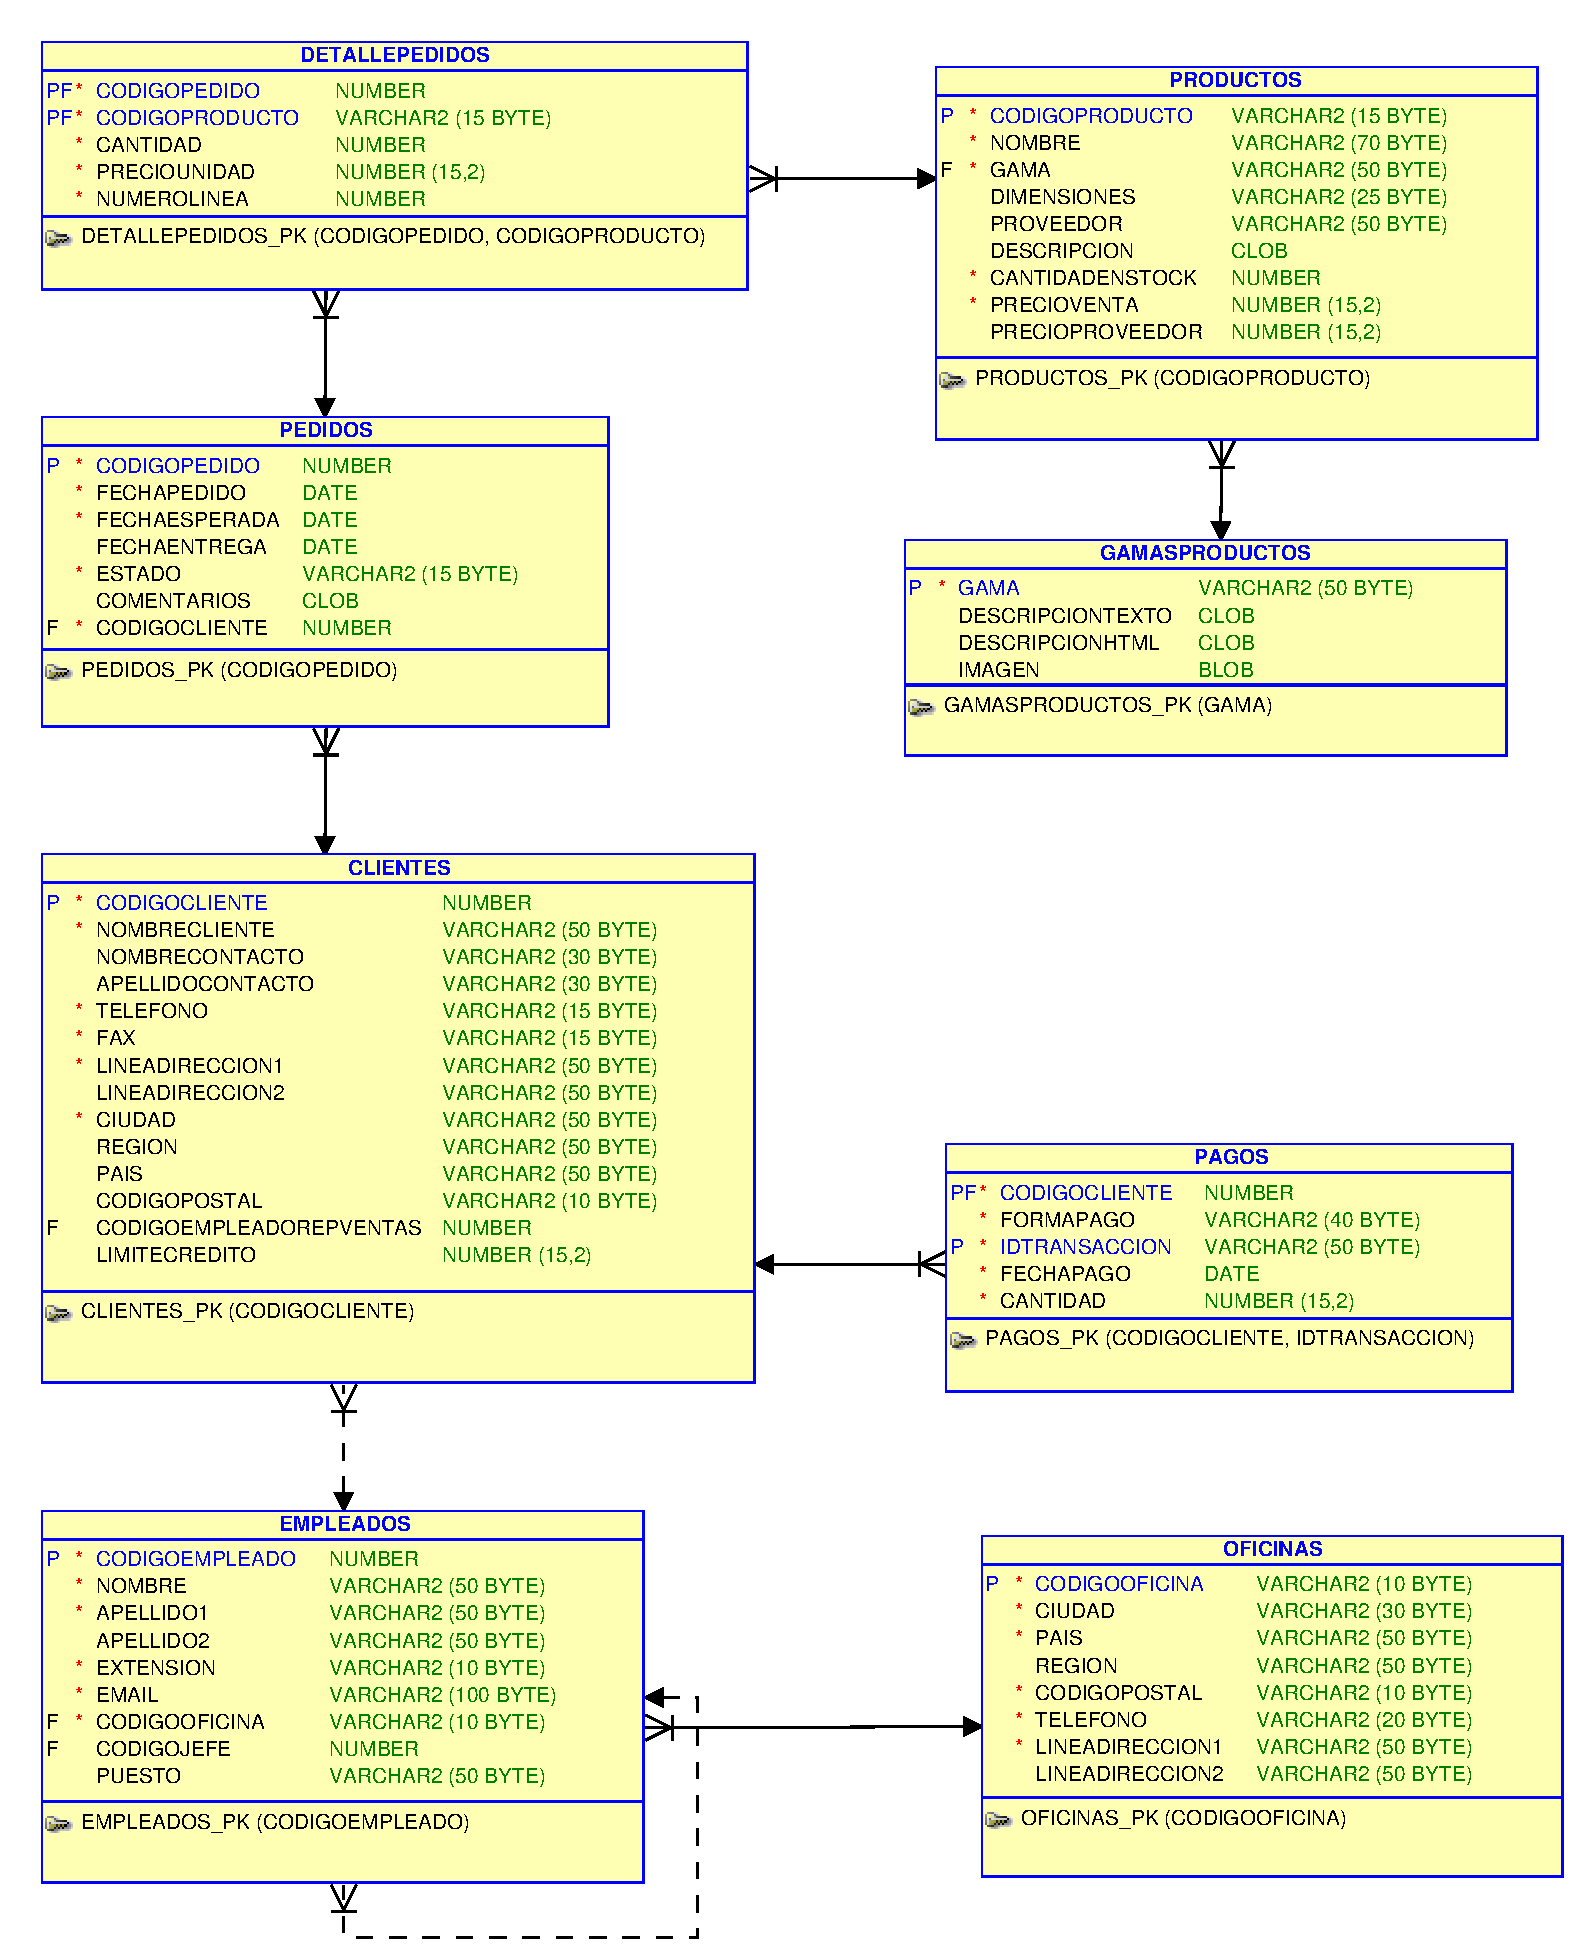
\includegraphics[width=.9\textwidth]{./jardineria.pdf}
  \end{center}
  \caption{Diagrama de la base de datos}\label{fig:esquema}
\end{figure}

\end{document}




